\chapter{研究背景}
\label{chap:background}

本章では既存のARナビゲーションシステムの現状と、その問題点を整理する。

\newpage



\section{ARによるナビゲーション支援システムの歴史}
ARによる表示をヘルプやナビゲーションシステムに利用する研究は90年代はじめから存在する。
初期の有名な例としてはプリンタのメンテナンス情報をARで表示するプロトタイプであるKARMA\cite{10.1145/159544.159587}や大学構内の案内をARで表示するナビゲーションシステムであるA Touring Machine\cite{629922}が挙げられる。
これらはヘッドマウントディスプレイを利用した物であるが、当時のヘッドマウントディスプレイは非常に大型で性能の限界もあり実用的とは言えなかった。

その後2000年代になりモバイル端末が普及するとGPSと方位などの情報をもとにカメラを通して周囲の情報をディスプレイに表示するアプリケーションが現れるようになった。
代表的な物としてWikitude\footnote{\textsf{https://www.wikitude.com/}}が挙げられる。
これらもモバイル端末の普及と合わせて話題となったが、位置測位精度の面で課題が残る物であった。



\section{ARによるナビゲーション支援の現状}
\label{current}
ARによるナビゲーション支援として実用化しているシステムを紹介し、その現状を解説する。



\subsection{Google MapsのARナビ機能}
Google\footnote{\textsf{https://google.com}}は2018年のGoogleI/O 2018で自社の開発する地図アプリケーションGoogle Maps\footnote{\textsf{https://www.google.com/maps}}にAR機能が追加されることを発表し、翌2019年5月に「ARナビゲーション」機能としてα版をリリースした。
この機能は目的地を地図で選択した上でARモードに切り替えることで起動でき、図\ref{fig:googleMapAr}のようにARで道案内を表示する機能である。
このアプリケーションではGPS(Global Positioning System)による位置情報や方位センサによる方位情報に加え、カメラで取得した周囲の景色の情報を元にユーザの位置と向きを判別し比較的高精度なAR表示を提供している。
一方で用途はあくまでもあくまでも目的地までの経路案内に限られており、GPSの届かない場所や周囲の景色による解析が難しい屋内では利用できないと言うデメリットが存在している。

\begin{figure}[H]
  \begin{center}
      \includegraphics[height=100mm]{images/google-maps-ar-mode.png}
  \end{center}
  \caption{Google MapsでのAR表示} \label{fig:googleMapAr}
\end{figure}



\subsection{遺跡・史跡のARナビゲーションアプリ}
日本国内の史跡ではマーカーベースのAR案内アプリケーションが複数採用されている。
これらのアプリケーションの大半は史跡の各地点にマーカーを設置し、その場所に関する解説や当時の様子を再現したCGをARで表示するという物である。
今回は一例として松山城址のナビゲーションアプリである「攻略 松山城」\footnote{\textsf{https://www.cadcenter.co.jp/works/archives/98}}を紹介する。
このアプリはARでの表示を用いながら松山城の歴史や仕組みをテキストや動画で解説するアプリである。
具体的には図\ref{fig:matsuyama_marker}のような専用のマーカーをアプリのカメラで読み込むことで、図\ref{fig:matsuyama_ar}のように解説動画のリンクを適切な位置に表示する。
広い史跡の中で実際の場所と見比べながら当時の様子や解説を参照できるこのようなアプリケーションはパンフレットなどと比べわかりやすく、有用であると言える。
一方でこのようなアプリケーションには以下のような問題点がある

\begin{itemize}
  \item マーカーの設置が面倒である\\
    表示したい場所ごとに図2.2のような大きなマーカーを設置しなければならずコストが高いと言える。
  \item アプリのダウンロード案内が別途必要になる\\
    案内専用のアプリとマーカーを利用しているためマーカーだけでなくアプリをダウンロードするための案内も必要になり、案内が冗長になってしまう。
    また特定の目的ごとに専用のアプリケーションを導入させる仕組みはユーザの負担となりうる。
\end{itemize}

\begin{figure}[H]
  \begin{minipage}{0.5\hsize}
    \centering
    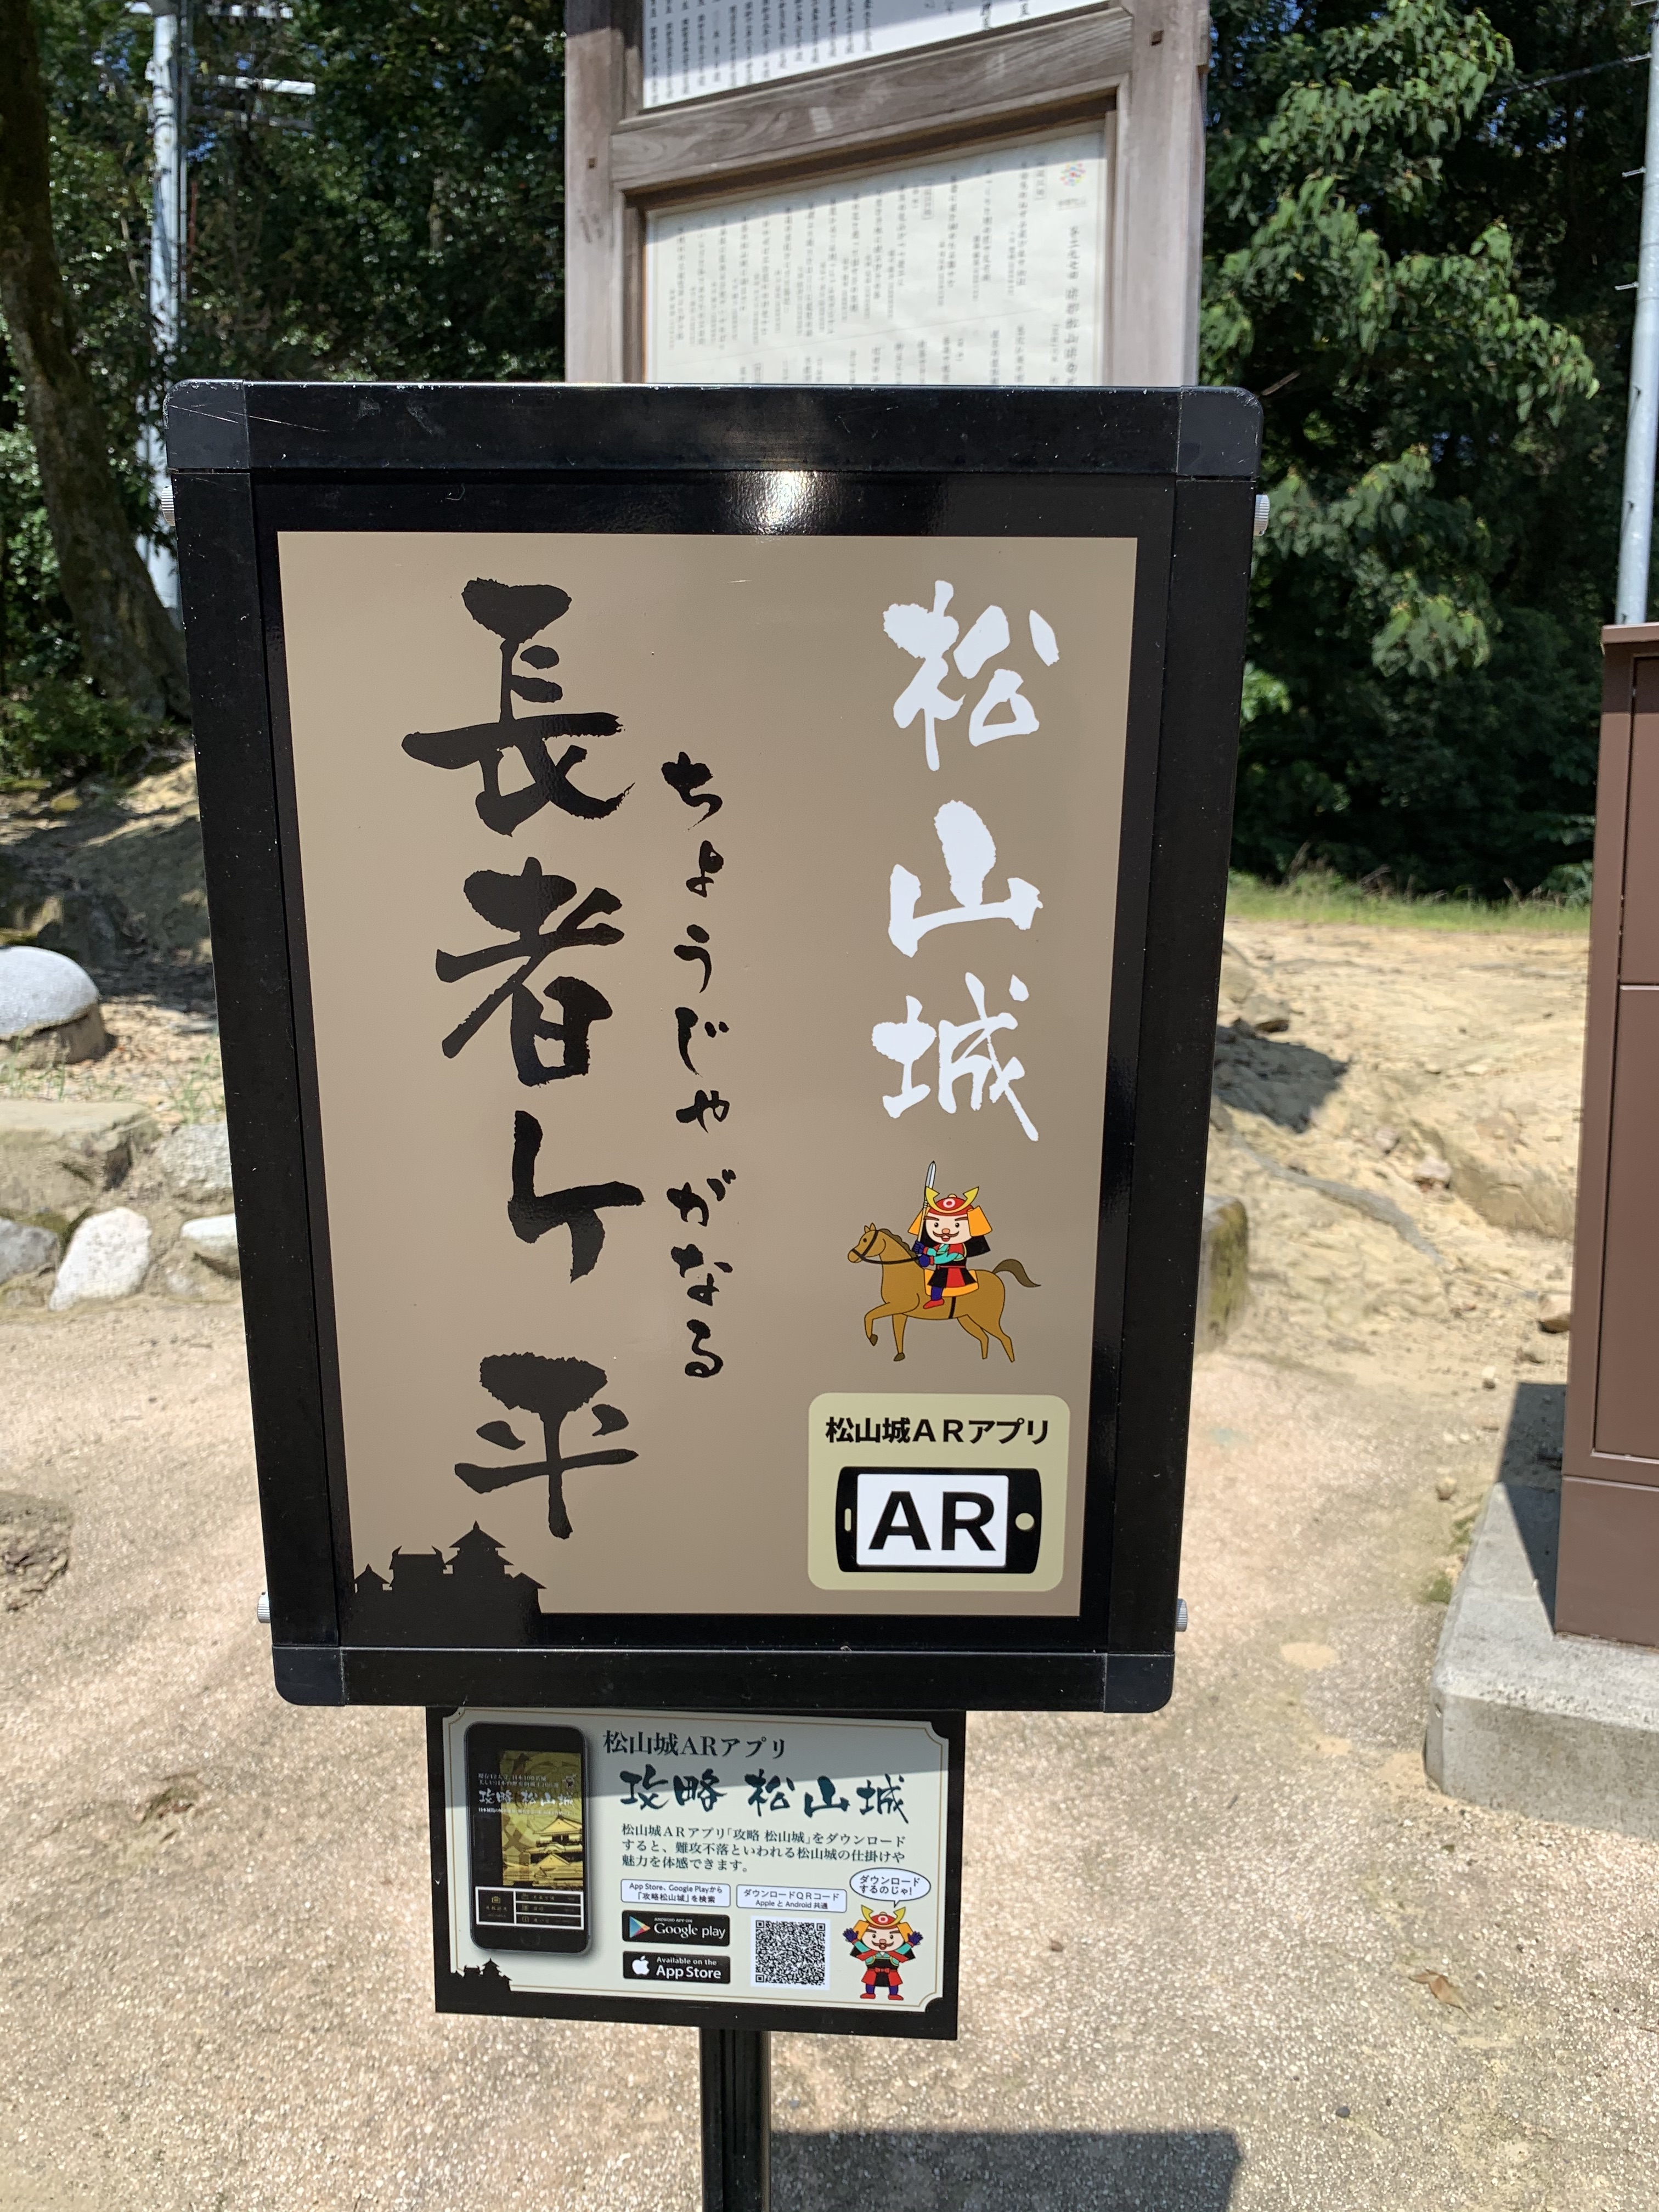
\includegraphics[width=70mm]{images/matsuyama_marker.jpg}
    \caption{専用のマーカー} \label{fig:matsuyama_marker}
  \end{minipage}
  \begin{minipage}{0.5\hsize}
    \centering
    \includegraphics[height=100mm]{images/matsuyama_ar.png}
    \caption{ARでの案内} \label{fig:matsuyama_ar}
  \end{minipage}
\end{figure}



\section{ARによるナビゲーションの問題点}
\label{problems}
前節で述べた現状を元に既存のARによるナビゲーションシステムの問題点を整理する。
ARのナビゲーションシステムには以下のような問題点がある。

\begin{itemize}
  \item 立ち上げるまでのインタラクションが面倒\\
    前節の「遺跡・史跡のARナビゲーションアプリ」のようにマーカーベースのARナビゲーションでは(1)設置されたマーカーを元にアプリを選択、(2)アプリを起動、(3)カメラでマーカーを中心に収めるという3ステップが必要になる。
    GPSと方位情報から位置測位を行うアプリケーションの場合、このような手順は必要ないが後述するように精度が悪く用途か限られるという問題がある。
  \item 位置測位の方法によって精度や用途が大きく限られる\\
    ARでのナビゲーションを行う際に多く用いられる位置測位の方法は、(1)マーカーを使う方法と(2)GPSによる座標検知と方位情報をあわせて利用する方法の2通りに大別される。
    (1)の場合マーカーが読み込めれば精度は高いが、ある程度の距離からカメラで十分認識できるサイズのマーカーを設置する必要がある。
    (2)の場合特別な設備は必要ないが精度面に疑問が残ることに加え、GPS電波の届く屋外に利用が限定される。
    前節で挙げたGoogleMapのAR機能ではGPSや方位情報に加えGoogleが撮影した道路の画像を元に補正を行い、精度を上げているが周囲の景色が登録されていない屋内での利用ができないという問題点は残る。
  \item 情報の登録・編集が面倒\\
    ARで単に目的地の位置を表示したり、決め打ったデータを表示するARナビゲーションアプリは多いが、情報の登録や編集の簡易さに焦点を置いた物は少ない。
    一方でARで表示したい情報は常に変化する可能性があり、今後も増加していくことが予想される。
    このような状況で一般ユーザが気軽に情報を登録編集できる環境を整えることは非常に重要である。
  \item 関連情報を参照・管理することができていない\\
    ARでの表示する情報が増えるにしたがってそれらを互いに参照したり、ドメインごとに管理するニーズは高まっていく。
    しかしながら既存のナビゲーションアプリではARで表示した情報同士を互いに参照して関連情報を表示したり、特定の分野でや条件でフィルターすることが難しい。
  \item 汎用性のあるアプリケーションがない\\
    上記のように「情報の登録・編集が面倒」、「関連情報を参照・管理することができていない」という問題点から特定の目的や分野に限ったARナビゲーションアプリは存在するものの、分野や目的を横断した汎用的ARナビゲーションアプリは開発されていない。
    そのため現状では目的や施設ごとにアプリケーションをユーザ側で切り替える必要があり、ARナビゲーションアプリが増えるほどユーザの負担は大きくなる。
    ユーザの目的やニーズは多岐に渡るためニーズごとにアプリケーションを分けて推薦するのではなく、様々な種類の情報を包括的に管理できるシステムが求められている。
    さらに目的や施設ごとにアプリケーションと情報が独立してしまうことで分野を横断したつながりを表現できないという問題点も生まれる。
\end{itemize}



\section{テキストや画像の進化}
前節で述べたとおりARによるナビゲーションには課題が多いが、ナビゲーションに利用しているテキストや画像などのメディアは計算機の進化とともに発展し、多くの問題点を克服している。

計算機上で利用されているテキストは、文字から内容を検索することが可能なため文書の参照や管理が格段に行いやすく、あらゆる文書が電子化されたテキストに置き換えられるようになった。
またWebやハイパーリンク等の技術によってより参照しやすくなったほか、別の文書を引用する等の再利用が可能になった。
さらにハイパーリンクを含んだ文書を手軽に作成・編集できるWiki\footnote{\textsf{}} が登場したことでより柔軟で活発なテキストによる知見の共有や情報の再利用が実現された。

同様に画像や地図などのメディアも電子化とWebの進歩により参照や管理が格段に行いやすくなった。
SNSや画像の管理が行えるクラウドウェアの普及により誰しもが写真を撮影し容易にWeb上にアップロード/公開することが可能になった。
このようにして公開された画像はURLによって一意に参照することができ、画像の再利用性は大きく高まった。
またGoogle Mapsのように、地理情報システム(GIS : Geographic Information System)が誰でも検索・参照可能な形でWebに公開されることで位置情報や地理情報を参照することが容易になった。

このような文書以外のメディアの進化に合わせ、近年の文書作成システムやWikiシステムは画像/音声/動画/地図といったマルチメディアを自在に埋め込む機能を持っている。

\section{Wikiとナビゲーションへの利用}
\subsection{Wiki}
WikiはWard Cunninghamが提案した不特定多数のユーザーが文書コンテンツを編集・管理するためのWebシステムである。
Wikiには以下のような特徴があり、情報を集積するコンテンツで多く活用される。
\begin{itemize}
  \item 独自の記法により編集が容易
  \item ブラウザ上で誰でもアクセスできる
  \item 文書間にリンクが張りやすく、個々の文書が高度に連携した文書群を作成しやすい
  \item 複数人が編集するため差分管理機能や同時編集機能を有する物もある
\end{itemize}

\subsection{現状のナビゲーションの限界}
第\ref{current}節で挙げたとおり現状のナビゲーションシステムは決まった目的地へ案内することを目的とする物が多い。
また目的地の検索機能を有していても、ユーザは能動的にキーワードを入力し目的地を絞り込む必要がある。
一方で、ナビゲーションを必要としているユーザの多くは漠然と達成したいことがあっても実際の目的地が分かっていない。
場合によっては達成したいこと自体が曖昧で言語化できていないこともある。
このような場合、ユーザに目的地を指定・検索させて案内をする現状のナビゲーションではユーザの目的を達成する事ができない。
ユーザ側に目的に関する知識や明確な意思がない場合に案内をできないことが現状のナビゲーションの限界であると言える。

\subsection{Wikiの有用性}
上記のようなナビゲーションの限界を解決するために必要な要素は以下であると考える。
\begin{enumerate}
  \item 幅広い分野の情報を提示することができる
  \item ユーザが周囲の情報を能動的に探索できる
  \item その結果自身の目的を明確化し目的地を確定できる。
\end{enumerate}
このような要素は情報管理ツールとしてWikiを利用すること満たすことができる。
Wikiは情報を分野で階層化・グルーピングすることなく一元的に管理する。
そのため1のように分野にとらわれない情報の提示が可能である。
またWikiはハイパーリンクによって文書間で参照しており、関連情報へのアクセスが容易である。
この特徴によって2のようにリンクをたどりながら自分の興味のある分野へページを遷移し、情報を探索することができる。
さらに探索によってユーザは周囲の情報を知識として吸収し、3のように目的を明確化することができる。
以上のような理由からナビゲーションにWikiを利用することで既存のナビゲーションの限界を打破した新しい形のナビゲーションが提供できると考える。


\section{NFC技術とインタラクション}
ARでのナビゲーションシステムには自身の位置情報やその場のコンテキスト情報が不可欠であり、一般的にそのような情報を瞬時に取得することは難しい。
一方NFCタグには以下のような特徴があり、実世界においてその場のコンテキスト情報や設置された物の情報を記述するのに便利である。

\begin{itemize}
  \item 電源がいらない
  \item 非常に薄く、小型
  \item IDやURLなどを記録するには十分な記憶容量を持つ
  \item 一枚あたり10円前後と安価
\end{itemize}

近年では多くのモバイル端末にNFCタグの読み取り機能が搭載されており、一般的なNFCタグであれば誰でも書き込まれた情報を瞬時に読み取ることができる。
さらに書き込むデータ形式によっては、モバイル端末でNFCタグの読み取るだけでWebページを開いたり、アプリを起動することが可能である。

このようなNFCタグの特徴は、現在一般的な用途である決済や在庫管理、家電操作などに加えナビゲーションシステムを補助するシステムとして有効であると考える。

一方でNFCタグは読み取る際に、読み取る機器をNFCタグにかなり近づける必要があるという制約がある。
この技術的制約は一般的にデメリットとして捉えられがちであるが、NFCタグを読み取ったタイミングでのユーザの持つ端末の位置はNFCタグとほぼ接していると確定できるとも言える。
つまりNFCタグに位置情報をもたせることができれば非常に小さい誤差でユーザの持つ端末をの位置を確定できることになる。
この特徴は第\ref{problems}節で述べた問題点の1つであるNFCの位置測位の問題を解決する。





\section{まとめ}
ARをナビゲーションとして利用するアイデアは以前から存在し、モバイル端末の普及と発展により実用段階に来ているプロダクトも増えている。
しかしながら第\ref{problems}節に上げた問題点を解決できていないため、汎用的なヘルプ・ナビゲーションとして利用されるに至っていない。
一方でナビゲーションに利用しているテキストや画像などのメディアは計算機上で積極的に応用されており、ハイパーリンクやWiki等の技術によって参照や再利用がより行いやすくなった。
また近年多くのモバイル端末に搭載されているNFC技術には第\ref{problems}節であげた問題点の一部を克服する可能性がある。
したがってARの正確な位置測位とコンテキスト情報の取得にNFCの技術を利用しつつ、ARで表示する情報の管理にWikiの手法を取り入れることで第\ref{problems}節に挙げた問題を解決できると考える。
次章では第\ref{problems}節に挙げたARナビゲーションシステムが持つ問題点を解決した、次世代のARナビゲーションシステム「HypAR Touch」を提案する。